\documentclass[a4paper, 12pt, one column, aas_macros]{article}

%% Language and font encodings. This says how to do hyphenation on end of lines.
\usepackage[english]{babel}
\usepackage[utf8x]{inputenc}
\usepackage[T1]{fontenc}
\usepackage{aas_macros}

%% Adds in official euro sign
\usepackage[official]{eurosym}

%% Sets page size and margins. You can edit this to your liking
\usepackage[top=1.3cm, bottom=2.0cm, outer=2.5cm, inner=2.5cm, heightrounded,
marginparwidth=1.5cm, marginparsep=0.4cm, margin=2.5cm]{geometry}

%% Useful packages
\usepackage{graphicx} %allows you to use jpg or png images. PDF is still recommended
\graphicspath{ {./images/} } % Sets base path for images
\usepackage[colorlinks=False]{hyperref} % add links inside PDF files
\usepackage{amsmath}  % Math fonts
\usepackage{amsfonts} % More fonts
\usepackage{amssymb}  % Symbols
\usepackage{subcaption} % Sub-figure captions

%% Citation package
\usepackage[nottoc]{tocbibind} %% Add refs to ToC
\usepackage[square,numbers]{natbib}
\bibliographystyle{dinat}
% \setcitestyle{authoryear,open={(},close={)}}

%% Change content and figure titles
\renewcommand{\contentsname}{Contents}
\renewcommand{\figurename}{Figure}

%% Begin document
\begin{document}

%% Create title page
\begin{titlepage}
    \title{
        Installing the power and temperature logger
    }
    \author{Stefan Schokker}
    \date{\today}
    \thispagestyle{empty}
\end{titlepage}

\maketitle
\thispagestyle{empty}

\newpage
\thispagestyle{empty}
\tableofcontents
\newpage

\setcounter{page}{1}
\section{Setup}
To continue where this project has left of, internet is definitely required. We use a hotspot to do everything that required an internet connection.\newline
The cluster also needs to be setup correctly. Make sure all the power connectors from the black PCB's are connected to the correct Raspberry Pi's. We labelled the Pi's from bottom to top: 0 - 3, with the highest up one being the "g" pi, or Grafana pi. In our setup we conected them to the PCB as follows:
\begin{table}[h]
\centering
\begin{tabular}{|l|l|}
\hline
Address & Pi \\ \hline
0x40 & 0 \\ \hline
0x41 & 1 \\ \hline
0x42 & 2 \\ \hline
0x43 & 3 \\ \hline
0x44 & G \\ \hline
\end{tabular}
\end{table}
\newline
With the addresses being on the following places:
\begin{figure}[h]
	\centering
	\begin{subfigure}[b]{0.4\linewidth}
    		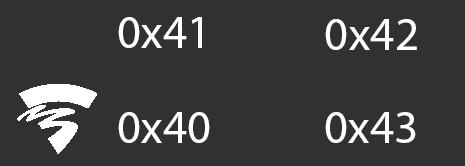
\includegraphics[width=\linewidth]{pcb-ina-0.png}
    		\caption{Bottom PCB}
    	\end{subfigure}
    \begin{subfigure}[b]{0.4\linewidth}
    		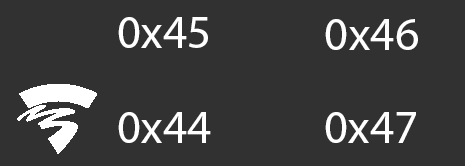
\includegraphics[width=\linewidth]{pcb-ina-1.png}
    		\caption{Top PCB}
    \end{subfigure}
    \caption{PCB INA connector layout, following page 18 of \url{http://www.ti.com/lit/ds/symlink/ina260.pdf}}
    \label{inapcb}
\end{figure}\newline
After that, make sure every Pi has it's own ethernet connection to the switch. If everything is setup correctly, it should work with the provided settings file "pis.xml" in the ina260 folder, the file will be required when starting the logger.\newline
\newline
NOTE:
\begin{itemize}
	\item In the current release of Debian Buster, the Pi picks only one of two interfaces (WiFi or Ethernet). Keep this in mind when trying to connect the Pi's to your hotspot.
\end{itemize}

\end{document}
